\section{Evaluation}
\label{section:evaluation}

In order to evaluate the scalability of our subsetter we performed both strong
and weak scaling tests.  All tests were performed on the franklin Cray-XT4
supercomputer\cite{franklin} located at NERSC\cite{NERSC}.  The performance
data collected was generated by custom wrappers to the functions we developed.
The IO wrappers perform barriers before and after each collective IO operation
is performed with the start and end time collected immediately after each
barrier.  Before program termination, the number of bytes written and read the
total time is collected on the zeroth process.  The profiling information
collects the number of times each function is called and how much time was
spent in each function and is only reported for the zeroth process and is
meant only as a general measure of performance.

\subsection{Strong Scaling}

\begin{figure}[!t]
\center
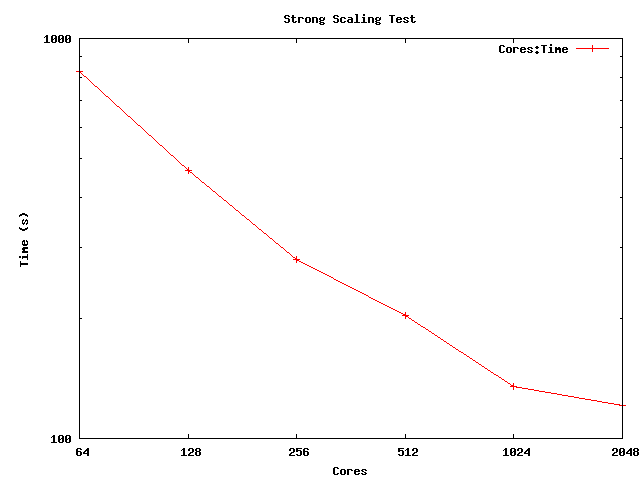
\includegraphics[width=3.5in]{plots/strong}
\caption{Strong Scaling Test}
\label{fig:strong}
\end{figure}

This test was run against 24 timesteps of an edge variable at a 4Km
resolution.  The total size of the data is XXX TB.  One timestep of the edge
variable is 17 GB (TODO: verify).  Figure \ref{fig:strong} shows the results
of the test.  The number of processors was doubled each run starting from 32.

\subsection{Weak Scaling}

TODO
